\chapter{Konzeption des Systems}
\label{chap:konzeption}

Die Konzeption des Systems bildet das Fundament für die spätere Implementierung und vereint moderne Technologien, um eine leistungsfähige und benutzerfreundliche Mitarbeitergesprächssoftware zu entwickeln. Im Zentrum der Konzeption stehen drei essenzielle Bereiche: das Design, die technischen Komponenten und die Datenarchitektur.

Das System zielt darauf ab, durch die Kombination von Frontend-Technologien wie React und Vite mit einem effizienten Backend auf Basis von .NET Core eine skalierbare und zuverlässige Plattform zu schaffen \cite{kirk2016data, microsoftDotNet}. Ergänzt wird dies durch eine relationale Datenbankstruktur, die mit Azure SQL realisiert wird, um eine robuste und sichere Speicherung sowie Verarbeitung der Gesprächsdaten zu gewährleisten \cite{azureDocumentation}.

Ein besonderer Fokus liegt auf der Interoperabilität mit bestehenden HR-Infrastrukturen. Durch den Einsatz von Microsoft Azure-Diensten wie Active Directory und Microsoft Graph wird eine nahtlose Integration ermöglicht, die nicht nur die Benutzerfreundlichkeit steigert, sondern auch die Effizienz datenbasierter Entscheidungsprozesse fördert \cite{microsoftAzure}. Die Architektur ist darauf ausgelegt, Visualisierungstools wie Donut- und Radarcharts zu integrieren, die eine intuitive und präzise Darstellung komplexer Daten unterstützen \cite{evergreen2016effective}.

Diese Konzeption stellt sicher, dass die verschiedenen Komponenten des Systems harmonisch zusammenwirken, um den Anforderungen moderner Arbeitsumgebungen gerecht zu werden und gleichzeitig die Grundlage für eine zukunftssichere Weiterentwicklung zu schaffen.

\section{Frontend-Architektur}
Das Frontend des Systems wird mit React und Vite geplant, um eine hohe Performance und schnelle Entwicklungszyklen zu gewährleisten. React dient als Kerntechnologie für die komponentenbasierte Architektur \cite{facebook2021react}, während Vite als moderner Build-Toolchain für eine optimale Ladezeit und Hot-Module-Replacement vorgesehen ist \cite{vite2022docs}. Zur Sicherstellung der Codequalität und Einhaltung von Best Practices wird ESLint integriert, um den Code auf potenzielle Fehler und Stilabweichungen zu überprüfen \cite{eslint2022guide}. Dies gewährleistet eine konsistente und wartbare Codebasis während der gesamten Entwicklungsphase.

\subsubsection*{Technische Grundlagen und Implementierung}
Das Frontend wird mit TypeScript geplant, um durch statische Typisierung die Lesbarkeit und Wartbarkeit des Codes zu erhöhen. Die Wahl der Technologien und Bibliotheken erfolgt gezielt, um die spezifischen Anforderungen des Projekts hinsichtlich Skalierbarkeit, Sicherheit und Benutzerfreundlichkeit zu erfüllen.

HTML bildet die Grundlage für die Strukturierung der Inhalte auf der Benutzeroberfläche, da es eine bewährte Basis für moderne Frameworks wie React bietet. React und react-dom werden für ihre komponentenbasierte Architektur gewählt, die eine effiziente Wiederverwendbarkeit von UI-Elementen ermöglicht \cite{facebook2021react}. 

Für das State-Management werden Redux Toolkit und Zustand evaluiert. Redux Toolkit wird für komplexere Datenflüsse verwendet, während Zustand aufgrund seiner Einfachheit für fokussierte Zustände gewählt wird. Zur Darstellung von Daten wird die Bibliothek ApexCharts geplant, da sie interaktive Diagramme wie Donut- und Radarcharts unterstützt \cite{apexchartsDoc}. 

\subsubsection*{Prototyping und Benutzerzentrierung} 
Für das Prototyping wird Figma verwendet, um frühzeitig Feedback zur Benutzeroberfläche einzuholen und diese iterativ zu verbessern. Dieser Ansatz sichert eine benutzerzentrierte Entwicklung, die den Anforderungen der Zielgruppe entspricht.

\begin{figure}[h!]
    \centering
    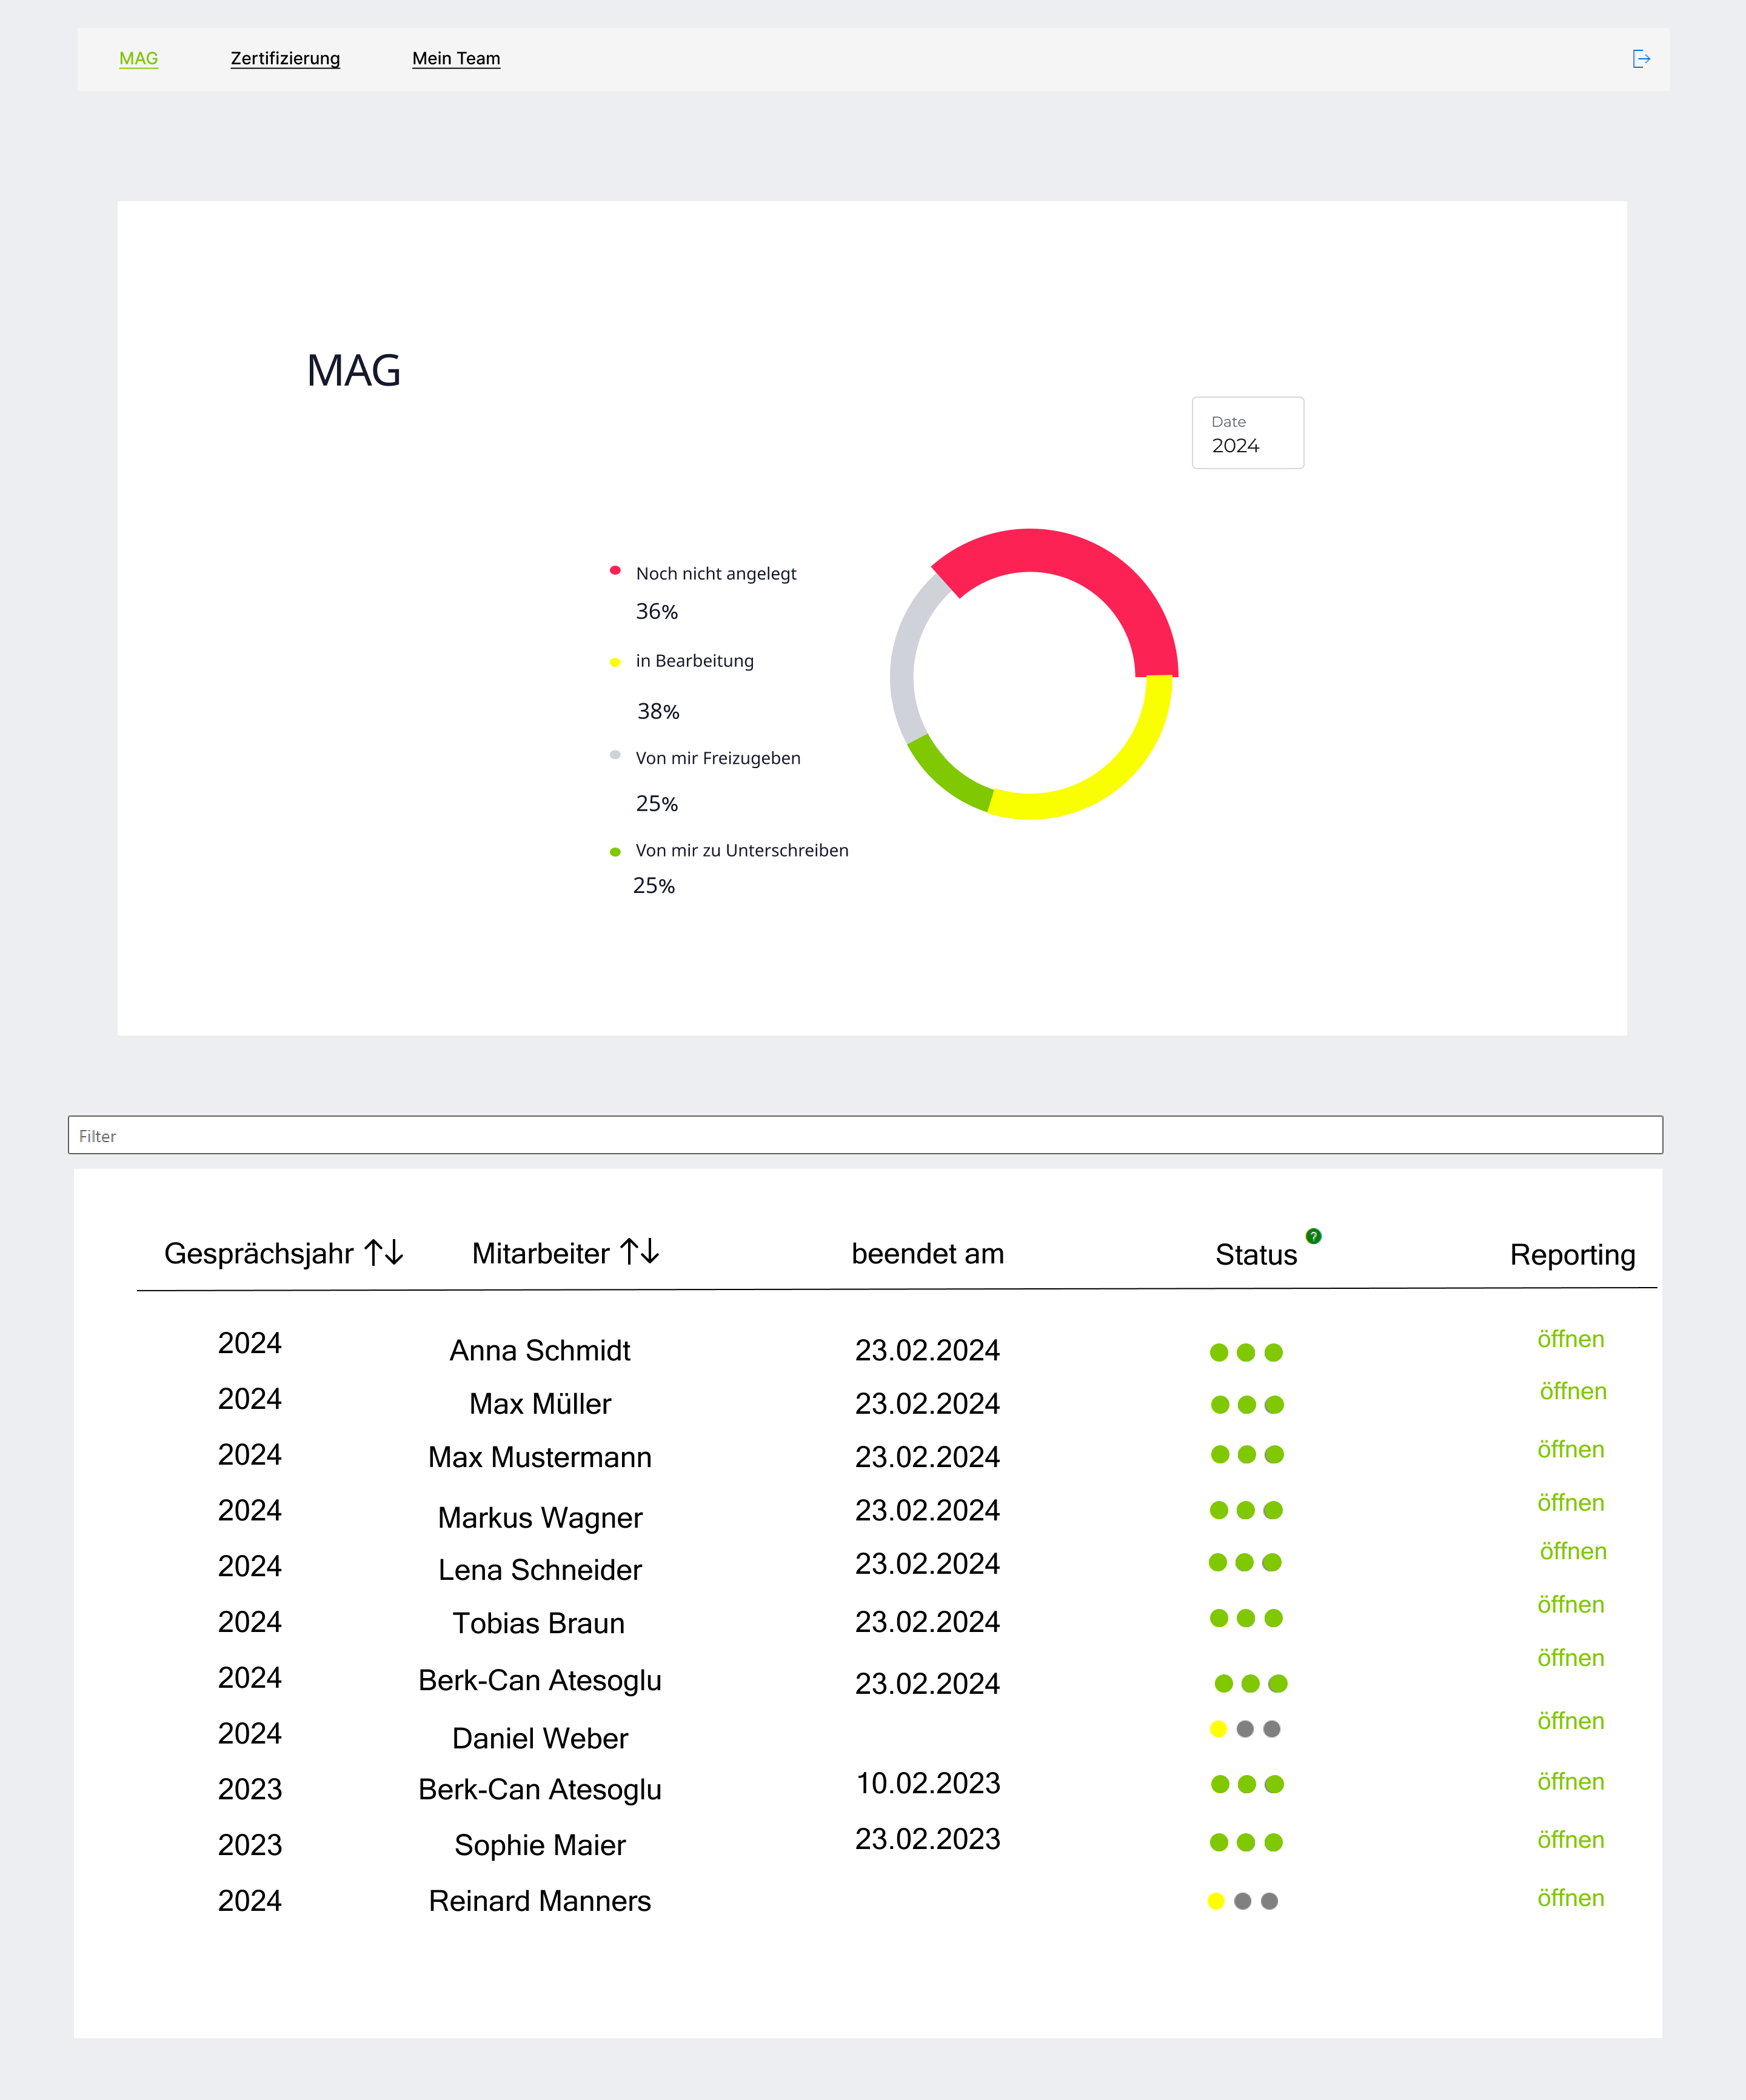
\includegraphics[width=1.2\textwidth]{images/Dashboard.png}
    \caption{Mockup der Hauptübersicht des Dashboards.}
    \label{fig:mockup1}
\end{figure}
\noindent
Abbildung \ref{fig:mockup1} zeigt das Mockup der Hauptübersicht des Dashboards. Diese Komponente ist der zentrale Einstiegspunkt für die Benutzer und bietet eine übersichtliche Darstellung der wichtigsten Kennzahlen und Statistiken. Ziel ist es, den Benutzern eine schnelle Orientierung zu ermöglichen, indem relevante Informationen, wie die Anzahl abgeschlossener Mitarbeitendengespräche oder ausstehender Aufgaben, prominent dargestellt werden. Interaktive Widgets ermöglichen es den Benutzern, tiefere Einblicke in spezifische Datenbereiche zu erhalten, ohne die Seite wechseln zu müssen.

\begin{figure}[h!]
    \centering
    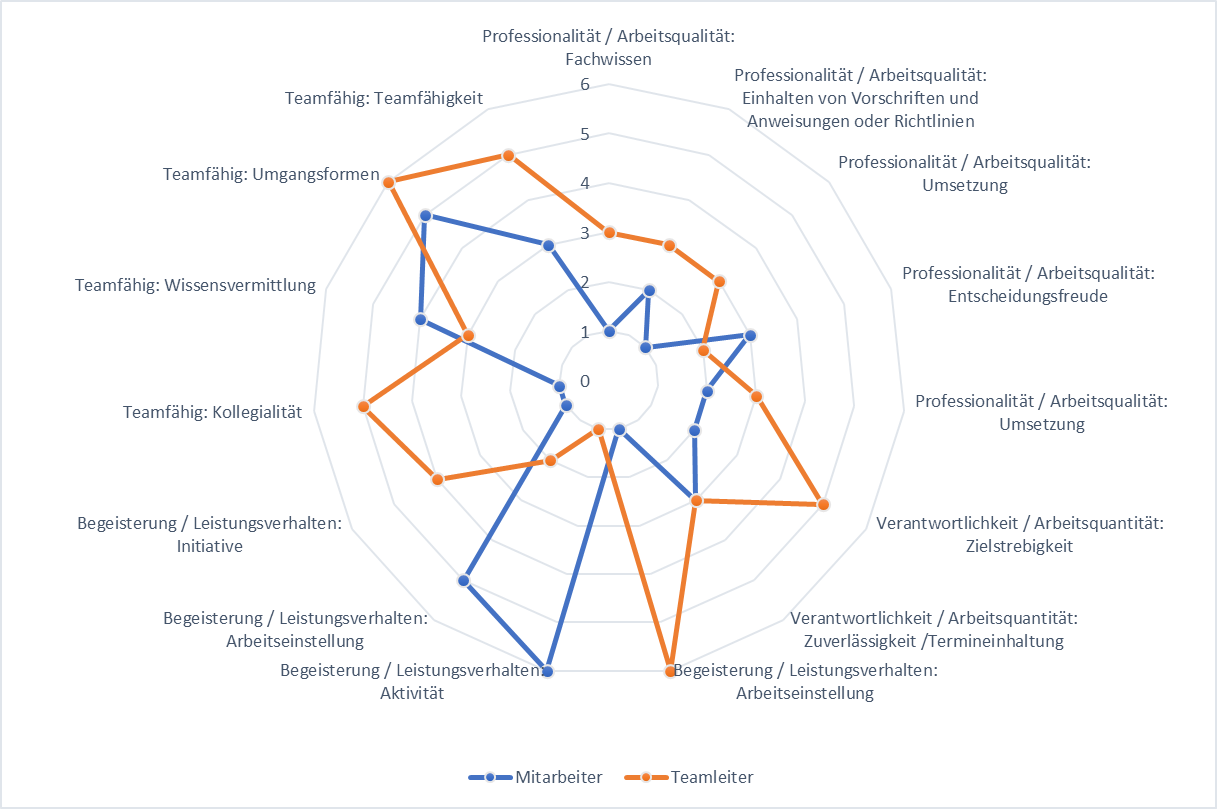
\includegraphics[width=1.2\textwidth]{images/radarchart.png}
    \caption{Mockup der Visualisierung vom Radarchart.}
    \label{fig:mockup2}
\end{figure}
\noindent
Abbildung \ref{fig:mockup2} illustriert die Visualisierung von Mitarbeitendengesprächsdaten in Form eines Radarcharts. Dieses Chart wurde gewählt, um die Bewertung einzelner Kompetenzen durch Mitarbeitende und Führungskräfte auf intuitive Weise vergleichbar zu machen. Durch die radiale Darstellung können Differenzen und Übereinstimmungen in verschiedenen Bewertungsdimensionen, wie Teamarbeit, Pünktlichkeit oder Innovation, auf einen Blick erkannt werden. Das Radarchart unterstützt die Benutzer bei der Analyse und Interpretation von Leistungsdaten, indem es komplexe Informationen in einer verständlichen visuellen Form präsentiert.

\begin{figure}[h!]
    \centering
    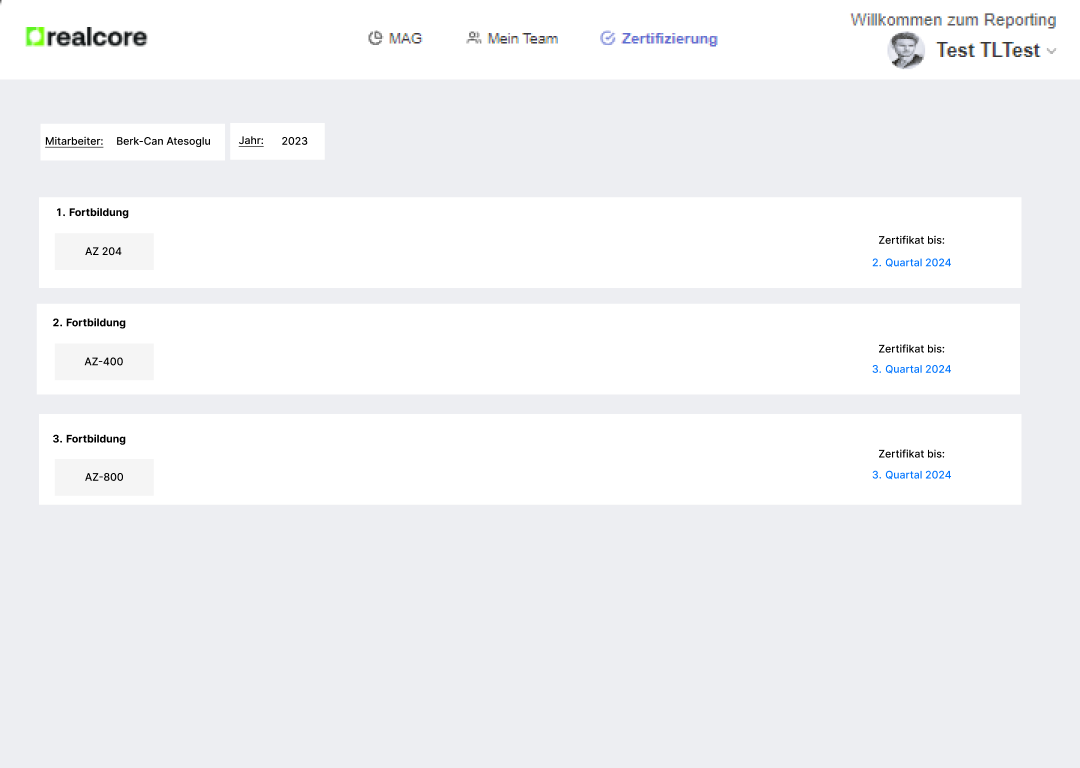
\includegraphics[width=1.2\textwidth]{images/Zertifikat.png}
    \caption{Mockup der Zertifikatsübersicht der Mitarbeiter.}
    \label{fig:mockup3}
\end{figure}
\noindent
Abbildung \ref{fig:mockup3} zeigt das Mockup der Zertifikatsübersicht der Mitarbeitenden. Diese Komponente bietet eine strukturierte Übersicht über erworbene Zertifikate, absolvierte Schulungen und deren Ablaufdaten. Der Zweck dieser Ansicht besteht darin, Führungskräften und HR-Teams eine einfache Nachverfolgung von Qualifikationen zu ermöglichen, sodass Weiterbildungsmöglichkeiten besser geplant werden können.


\subsubsection*{Entwicklungsprozesse und DevOps} 
Das Projekt wird mittels Azure Pipelines in eine CI/CD-Pipeline integriert. Dies ermöglicht automatisierte Tests und Deployments des Frontends in verschiedene Umgebungen. Azure Pipelines bietet eine nahtlose Integration in das Microsoft-Ökosystem und erleichtert die Verbindung mit Azure-Diensten wie Azure Repos und Azure Artifacts \cite{microsoftAzurePipelines}. Diese enge Integration reduziert die Komplexität der Konfiguration und erhöht die Effizienz im Entwicklungsprozess. Zudem unterstützt Azure Pipelines eine exzellente Skalierbarkeit, da Cloud-basierte Build-Agenten flexibel hinzugefügt werden können, was insbesondere bei größeren Projekten von Vorteil ist \cite{ciCdScalability}.

Zusätzlich wird Docker für die Containerisierung eingesetzt, um eine konsistente Entwicklungs- und Produktionsumgebung sicherzustellen. Im Vergleich zu virtuellen Maschinen zeichnet sich Docker durch eine geringere Ressourcennutzung und schnellere Startzeiten aus, wodurch Entwicklungszyklen beschleunigt werden \cite{dockerVsVm}. Docker ermöglicht zudem eine einfache Skalierung und Portabilität der Anwendungen, da Container unabhängig von der zugrunde liegenden Infrastruktur betrieben werden können \cite{dockerScalability}.

Die Kombination aus Azure Pipelines und Docker bietet eine zukunftssichere DevOps-Lösung, die sowohl für kleine Teams als auch für große Unternehmen geeignet ist. Diese Technologien fördern eine schnelle, zuverlässige und kontinuierliche Bereitstellung von Software und sind daher anderen Ansätzen in Bezug auf Effizienz und Integration überlegen \cite{azureDockerIntegration}.



\section{Backend-Architektur}
Die Backend-Architektur stellt eine zentrale Komponente in der Planungsphase des Systems dar und soll eine robuste und skalierbare Grundlage für die Verarbeitung und Speicherung der Daten bieten. Verschiedene Technologien und Ansätze wurden evaluiert, um die effizienteste Lösung für die Anforderungen des Projekts zu identifizieren.

\subsubsection*{Zentrale Dienste und Technologien}
Die geplante Backend-Architektur basiert auf einer modularen Struktur, die mehrere essenzielle Dienste und Technologien integriert. Ein zentrales Element ist der Azure Service Bus, der für die Verarbeitung und Synchronisation von Nachrichten zwischen den verschiedenen Systemkomponenten vorgesehen ist. Das Publish-Subscribe-Muster, das durch den Azure Service Bus unterstützt wird, reduziert die Kopplung zwischen Systemkomponenten und ermöglicht eine flexible Integration neuer Komponenten sowie eine hohe Skalierbarkeit \cite{azureServiceBus2024}.

\begin{figure}[H]
    \centering
    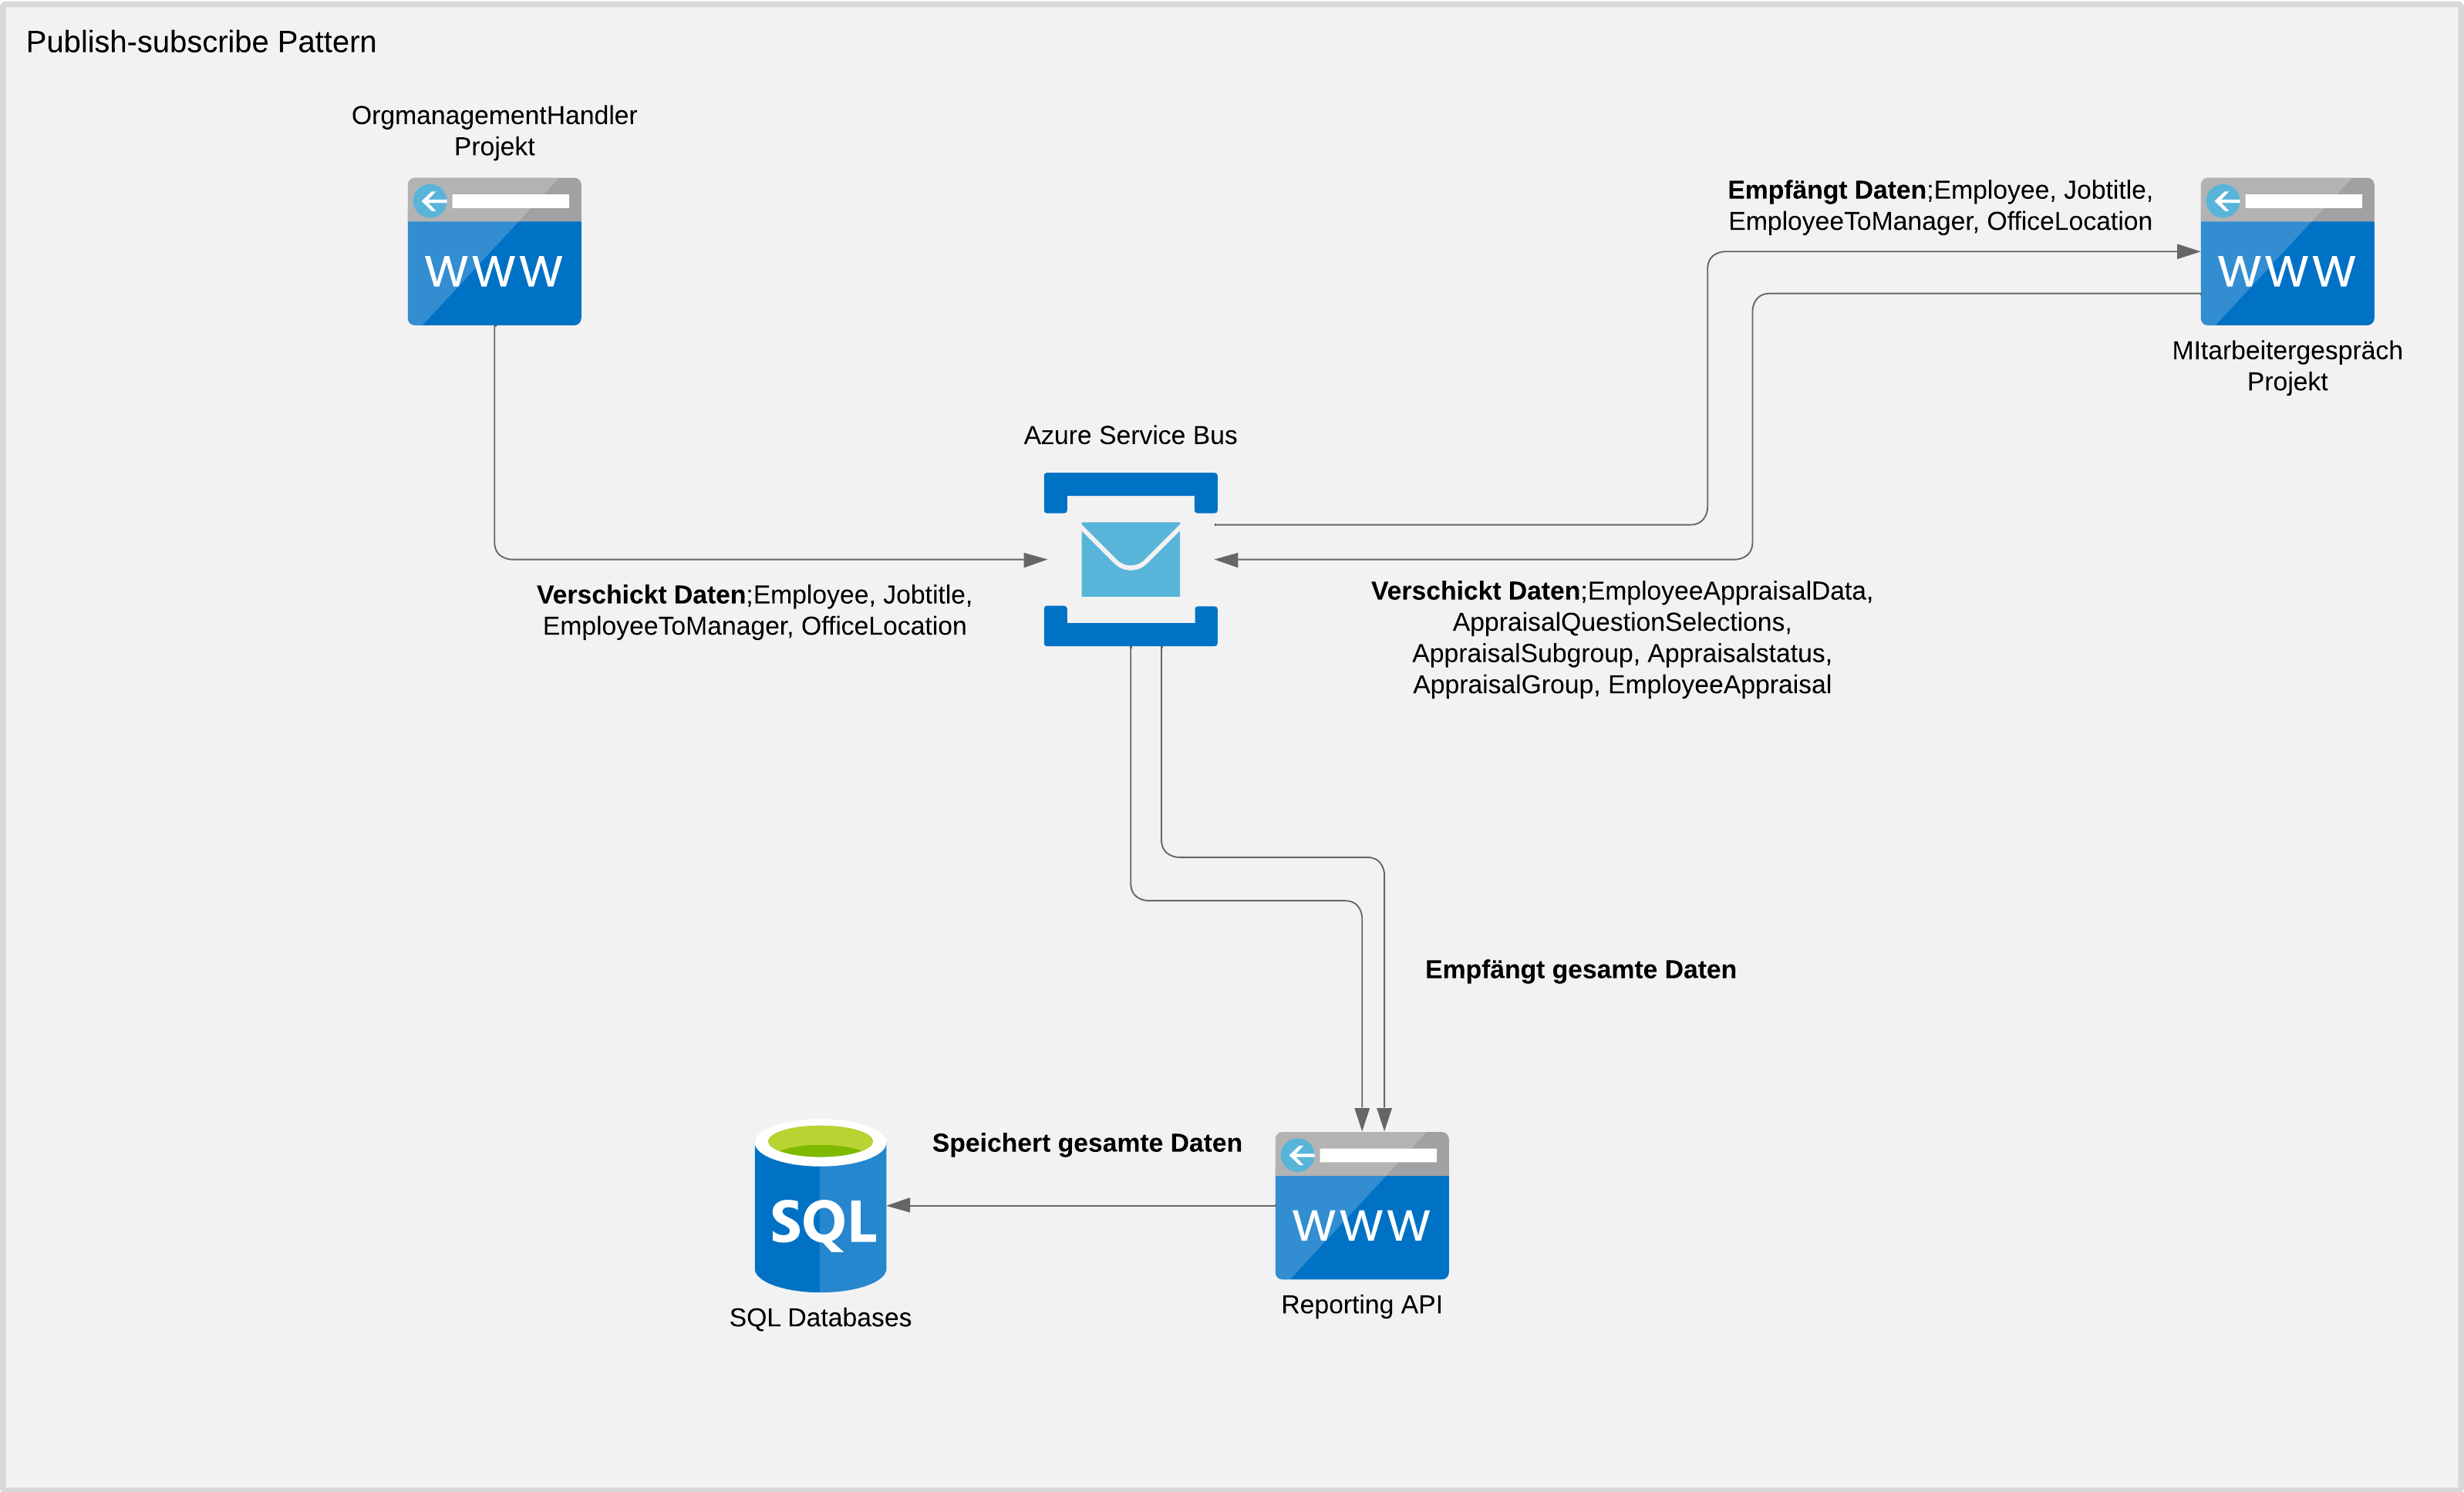
\includegraphics[width=1.0\textwidth, keepaspectratio]{images/Azure (2019) framework - Page 1.png}
    \caption{Architektur des Azure Service Bus im Publish-Subscribe-Pattern.}
    \label{fig:azure_bus_architecture}
\end{figure}

Das in Abbildung~\ref{fig:azure_bus_architecture} dargestellte Publish-Subscribe-Muster bildet die Grundlage für die Kommunikation zwischen den verschiedenen Systemkomponenten. Der Azure Service Bus erlaubt es, Nachrichten gezielt über sogenannte Topics an registrierte Subskriptionen zu verteilen. Diese Architektur bietet mehrere Vorteile, darunter eine bessere Skalierbarkeit und die flexible Integration neuer Komponenten. Besonders für Systeme mit hohem Kommunikationsaufkommen oder solchen, die in dynamischen Umgebungen weiterentwickelt werden müssen, ist diese Lösung optimal.

Im vorliegenden Systemdesign spielt der Azure Service Bus eine zentrale Rolle, indem er Daten aus zwei verschiedenen Anwendungen empfängt: dem Orgmanagement-Handler und dem Mitarbeitendengesprächsprojekt (MAG). Die vom Orgmanagement-Handler übermittelten Daten umfassen Informationen wie \textit{Employee}, \textit{Jobtitle}, \textit{EmployeeToManager} und \textit{OfficeLocation}. Diese Daten sind essenziell, um eine aktuelle und konsistente Übersicht über die Organisationsstruktur zu gewährleisten. Ergänzend dazu liefert das Mitarbeitendengesprächsprojekt zusätzliche Daten, darunter \textit{EmployeeAppraisalData}, \textit{AppraisalQuestionSelections}, \textit{AppraisalSubgroup}, \textit{AppraisalStatus}, \textit{AppraisalGroup} und \textit{EmployeeAppraisal}, die für die Analyse und Visualisierung der Mitarbeitendengespräche von zentraler Bedeutung sind.

Wie in Abbildung~\ref{fig:azure_bus_architecture} dargestellt, erfolgt die Übermittlung der Daten zunächst an den Azure Service Bus, wo sie in spezifischen Topics organisiert werden. Die Subskriptionen, wie die SQL-Datenbank oder das Reporting API, greifen gezielt auf diese Topics zu, um die benötigten Informationen zu extrahieren. Dieser Ansatz reduziert die Kopplung zwischen den Systemen erheblich und ermöglicht eine einfache Erweiterung oder Anpassung der Datenströme ohne Änderungen an bestehenden Komponenten vorzunehmen. So können beispielsweise neue Datenquellen oder Subskriptionen hinzugefügt werden, ohne dass dies Auswirkungen auf die bereits existierenden Abläufe hat.

Der gesamte Prozess beginnt mit der Übermittlung der Organisationsdaten, wie Informationen über Mitarbeiter, Jobtitel und Zuordnungen von Führungskräften, durch den Orgmanagement-Handler. Parallel dazu liefert das Mitarbeitendengesprächsprojekt relevante Gesprächsdaten, die über den Azure Service Bus an die registrierten Subskriptionen verteilt werden. Die SQL-Datenbank speichert sämtliche Daten, während das Reporting API sie verarbeitet und für die Visualisierung aufbereitet. Durch diese flexible und skalierbare Architektur wird nicht nur eine effiziente Verarbeitung der Daten gewährleistet, sondern auch eine hohe Anpassungsfähigkeit für zukünftige Anforderungen geschaffen. Der Azure Service Bus fungiert hierbei als zentrales Kommunikationsmedium, das eine nahtlose Integration und Synchronisation zwischen den verschiedenen Systemkomponenten sicherstellt und dabei gleichzeitig die Performance des gesamten Systems optimiert.


Für den Datenbankzugriff wird Entity Framework Core evaluiert, das im Vergleich zu Tools wie Dapper eine höhere Abstraktionsebene und eine nahtlose Integration mit .NET Core bietet \cite{entityFrameworkCore2020}. Durch diese Wahl wird die Verwaltung von Datenbankoperationen deutlich vereinfacht, ohne dass die Performance darunter leidet. 

Zusätzlich sind automatisierte Hintergrundjobs Teil des Konzepts, die für Aufgaben wie das Versenden von Benachrichtigungen oder das Berechnen aggregierter Daten verantwortlich sind. Diese Hintergrundprozesse werden ebenfalls mithilfe des Azure Service Bus orchestriert, was eine zuverlässige und asynchrone Verarbeitung gewährleistet \cite{backgroundTasks2017}.

Durch die sorgfältige Auswahl und Integration dieser Technologien wird eine flexible, sichere und skalierbare Backend-Architektur geschaffen, die sowohl aktuellen als auch zukünftigen Anforderungen gerecht wird.


\subsubsection*{Technologien und Abhängigkeiten}
Das Backend verwendet moderne Technologien und Bibliotheken, um die Anforderungen an Sicherheit, Performance und Skalierbarkeit zu erfüllen. Die Auswahl dieser Technologien erfolgte nach einem detaillierten Vergleich mit alternativen Lösungen, um die optimale Grundlage für das System zu schaffen.

AutoMapper wurde für die Abbildung von Datenmodellen und Data Transfer Objects (DTOs) gewählt. Es bietet eine intuitive Konfiguration und automatisierte Abbildung, die den Entwicklungsaufwand deutlich reduziert und die Lesbarkeit des Codes verbessert \cite{automapperDocs}. Im Vergleich zu manuellen Mappings, die fehleranfällig und zeitintensiv sind, minimiert AutoMapper den Boilerplate-Code erheblich. Eine mögliche Alternative wie MapStruct ist zwar leistungsfähig, richtet sich jedoch an Java-basierte Systeme und bietet keine vergleichbare Integration für .NET.

Für die Messaging-Lösungen wurde MassTransit in Kombination mit MassTransit.Azure.ServiceBus.Core ausgewählt. Diese Bibliotheken ermöglichen eine einfache Implementierung des Publish-Subscribe-Musters und bieten eine nahtlose Integration mit dem Azure Service Bus \cite{masstransit2021}. RabbitMQ, eine oft genutzte Alternative, bietet zwar ähnliche Funktionalitäten, erfordert jedoch eine aufwendigere Konfiguration und Wartung, insbesondere in Cloud-Umgebungen. MassTransit überzeugt zudem durch eine bessere Integration mit .NET Core, wodurch Entwicklungszeit eingespart wird.

Zur Authentifizierung und Autorisierung wurde die Nutzung von JSON Web Tokens (JWT) mittels Microsoft.AspNetCore.Authentication.JwtBearer festgelegt. JWTs bieten eine skalierbare und serverunabhängige Lösung, die ideal für verteilte Systeme geeignet ist \cite{jwtAuthDocs}. Im Vergleich zu klassischen Session-Management-Ansätzen, die auf eine zentrale Speicherung angewiesen sind und weniger skalierbar sind, ist JWT eine leichtgewichtige und effiziente Alternative. Andere Authentifizierungsmethoden wie OAuth mit Access Tokens können zwar in bestimmten Szenarien sinnvoll sein, bringen in diesem Kontext jedoch eine unnötige Komplexität mit sich.

OData wurde implementiert, um erweiterten Abfragefunktionen wie Filterung, Paging und Sortierung direkt auf API-Ebene zu ermöglichen. Diese Funktionen reduzieren die Komplexität im Frontend und optimieren die Datenverarbeitung, da weniger Daten transferiert und verarbeitet werden müssen \cite{odata2022}. Traditionelle REST-APIs bieten diese erweiterten Funktionen nicht von Haus aus, sondern erfordern zusätzliche Implementierungen, die die Komplexität und den Entwicklungsaufwand erhöhen. OData bietet hier eine standardisierte und leistungsfähigere Lösung.

Die sorgfältige Auswahl dieser Technologien gewährleistet eine robuste und skalierbare Backend-Architektur. Durch die Integration bewährter Frameworks und Bibliotheken wird eine effiziente Entwicklung ermöglicht, die sowohl den aktuellen Anforderungen als auch zukünftigen Erweiterungen gerecht wird.

\section{Datenbankdesign}
Die Konzeption der Datenbank ist ein zentraler Bestandteil der Systemplanung, da sie das Rückgrat für die Speicherung und Verarbeitung großer Datenmengen bildet. Nach der Prüfung von PostgreSQL und MySQL fiel die Entscheidung auf Microsoft SQL Server, da es eine nahtlose Integration mit Azure-Diensten und umfangreiche Sicherheitsfunktionen bietet.

\subsection{Beziehungsmodell}
Das Beziehungsmodell der geplanten Datenbank basiert auf einem relationalen Design, das eine effiziente Speicherung, Abfrage und Verarbeitung der Daten ermöglicht. Dieses Modell orientiert sich an etablierten Prinzipien der relationalen Datenbanktheorie, wie sie erstmals von Codd definiert wurden \cite{codd1970relational}. Abbildung \ref{fig:db_er_model} zeigt das ER-Diagramm der geplanten Datenbankstruktur, das die Entitäten und ihre Beziehungen detailliert darstellt. Das Design umfasst mehrere zentrale Tabellen, die eng miteinander verbunden sind, um eine konsistente und skalierbare Datenarchitektur sicherzustellen. Die Tabelle \textit{Employee} speichert Stammdaten wie Namen, Rollen und Standorte der Mitarbeitenden und ist mit der Tabelle \textit{EmployeeAppraisal} verknüpft, um Daten zu individuellen Mitarbeitendengesprächen zu referenzieren. Die Tabelle \textit{EmployeeAppraisal} enthält dabei spezifische Informationen zu den Gesprächen, wie Datum, Status und beteiligte Personen, und ist zusätzlich mit \textit{AppraisalGroup} und \textit{AppraisalQuestion} verbunden, um eine logische Strukturierung der Bewertungsfragen zu ermöglichen. 

Ein besonderer Fokus des Designs liegt auf der Normalisierung bis zur dritten Normalform (3NF), um Redundanzen zu vermeiden und die Datenkonsistenz zu sichern. Durch die Trennung der Entitäten in eigene Tabellen werden potenzielle Anomalien bei Einfüge-, Lösch- oder Aktualisierungsvorgängen vermieden \cite{elmasri2020fundamentals}. Indizes auf häufig abgefragten Attributen, wie Primär- und Fremdschlüsseln, werden implementiert, um die Abfrageleistung zu optimieren. Das gewählte relationale Modell wurde gegenüber anderen Datenbankmodellen, wie NoSQL-Datenbanken, evaluiert. Während NoSQL-Datenbanken wie MongoDB Vorteile in der Verarbeitung unstrukturierter Daten bieten, eignen sie sich weniger für stark strukturierte und transaktionsintensive Anwendungen wie dieses System. Relationale Datenbanken hingegen garantieren durch die ACID-Eigenschaften (Atomicity, Consistency, Isolation, Durability) eine hohe Sicherheit und Zuverlässigkeit der Daten \cite{stonebraker2010nosql}.

Die geplante Datenbankstruktur ist zudem flexibel gestaltet, um zukünftige Erweiterungen zu erleichtern. Beispielsweise könnten zusätzliche Tabellen für Schulungsdaten oder Leistungsbewertungen eingeführt werden, ohne die bestehende Architektur wesentlich zu verändern. Um datenintensive Anwendungen zu unterstützen, könnten in der Zukunft Materialized Views verwendet werden, die komplexe Abfragen beschleunigen, indem Zwischenergebnisse vorab berechnet und gespeichert werden \cite{gupta1995materialized}. Das relationale Design kombiniert klare Strukturierung, effiziente Abfragen und flexible Erweiterungsmöglichkeiten und stellt somit sicher, dass die Datenbank sowohl den aktuellen Anforderungen entspricht als auch zukunftssicher bleibt.

\begin{sidewaysfigure}
    \centering
    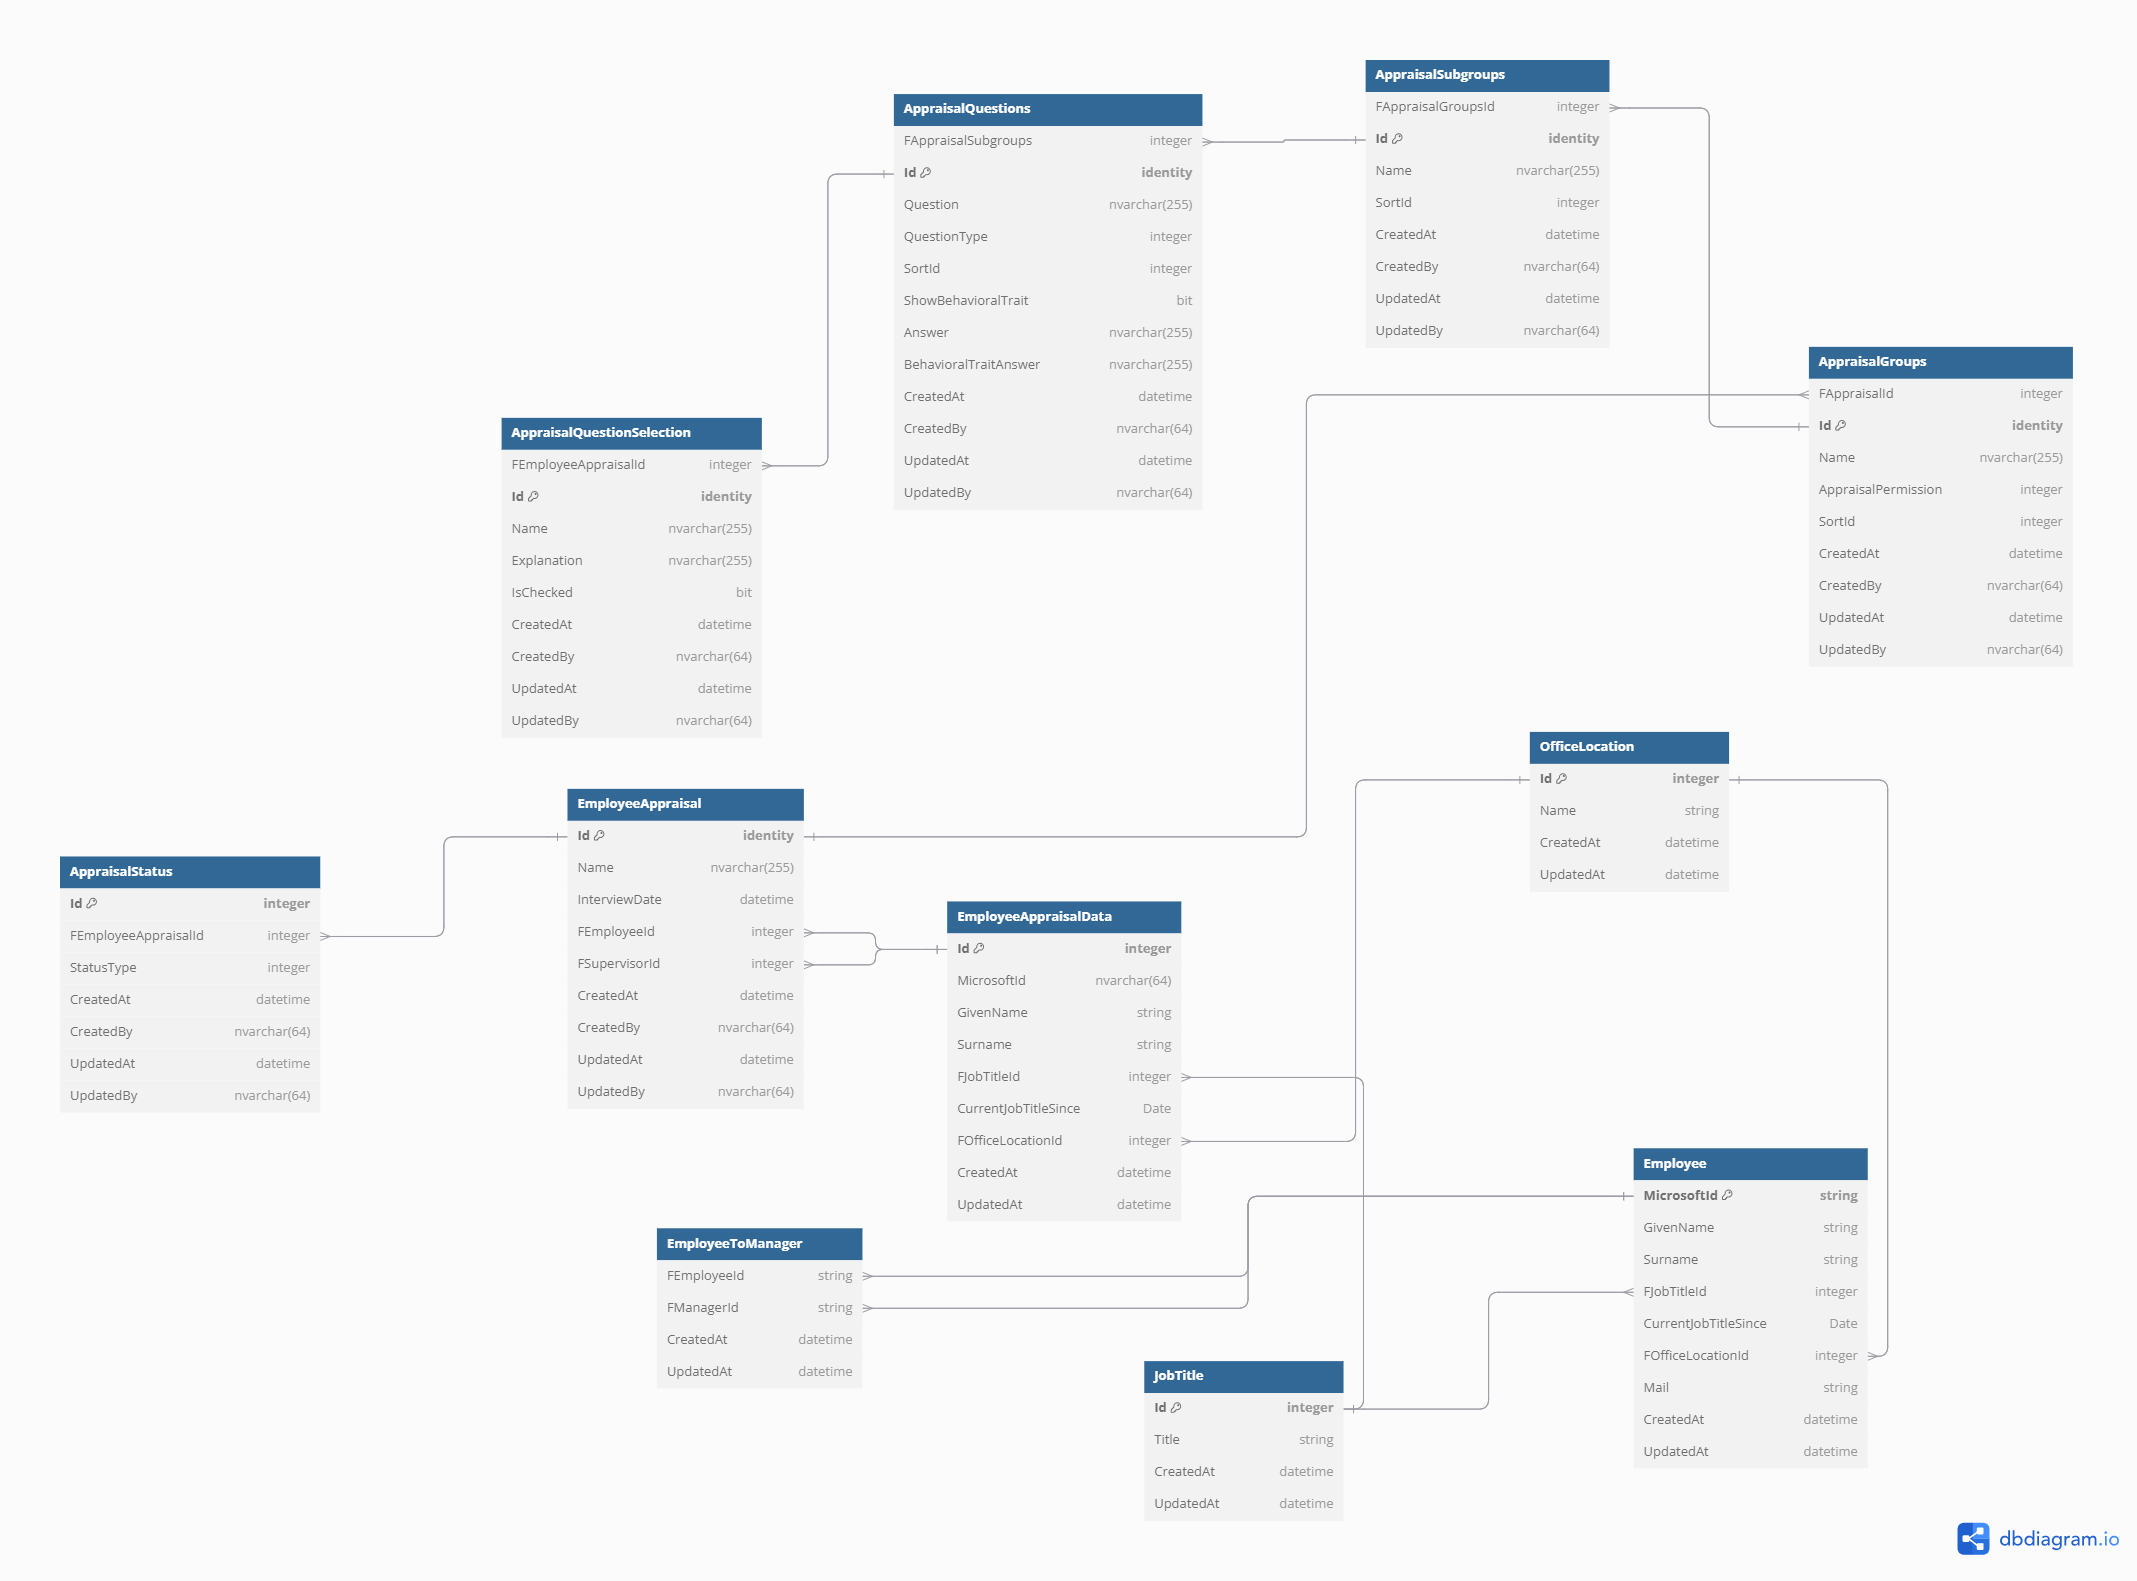
\includegraphics[width=1.1\textheight]{images/er_modell_design.png}
    \caption{ER-Diagramm der geplanten Datenbankstruktur.}
    \label{fig:db_er_model}
\end{sidewaysfigure}


\section{Sicherheitskonzept}

Das Sicherheitskonzept der Anwendung basiert auf einer modernen und robusten Authentifizierungs- und Autorisierungslösung, die durch die Integration von Azure Active Directory (Azure AD) realisiert wird. Ziel ist es, den Zugriff auf sensible Daten und Funktionen effektiv zu schützen und gleichzeitig eine einfache Benutzererfahrung zu gewährleisten.

Die Benutzeranmeldung erfolgt im Frontend mithilfe der Microsoft Authentication Library (MSAL). Hierbei wird ein sicherer Authentifizierungsprozess implementiert, bei dem sich Benutzer über ihre Microsoft-Konten anmelden. Nach erfolgreicher Authentifizierung wird ein JSON Web Token (JWT) generiert. Dieses Token enthält die Identität des Benutzers sowie die entsprechenden Berechtigungen. Die relevanten Berechtigungen werden durch sogenannte Scopes definiert, welche den Zugriff auf bestimmte APIs regeln. Dieses Token wird im \texttt{sessionStorage} des Browsers gespeichert und bei jeder Anfrage an das Backend im HTTP-Header als \texttt{Authorization: Bearer <Token>} übermittelt.

Das Backend überprüft die Gültigkeit des JWTs bei jeder Anfrage, um sicherzustellen, dass nur autorisierte Benutzer auf die Ressourcen zugreifen können. Dazu wird das Token mit Azure AD validiert. Falls das Token ungültig oder abgelaufen ist, wird die Anfrage abgelehnt, und der Benutzer erhält eine \texttt{401 Unauthorized}-Antwort. Zusätzlich wird sichergestellt, dass alle API-Endpunkte standardmäßig durch ein Autorisierungskonzept geschützt sind. Dies wird durch die Konfiguration eines zentralen Autorisierungsfilters realisiert, der festlegt, dass nur authentifizierte Benutzer Zugriff auf die Endpunkte haben.

Ein weiterer wesentlicher Aspekt des Sicherheitskonzepts ist die Verschlüsselung der Datenübertragung. Alle Anfragen und Antworten zwischen dem Frontend und Backend erfolgen ausschließlich über HTTPS, um sicherzustellen, dass die Kommunikation verschlüsselt ist und nicht von unbefugten Dritten abgefangen werden kann. Dadurch wird die Vertraulichkeit der übertragenen Daten gewährleistet.

Um die Sicherheit weiter zu erhöhen, werden die Tokens nicht im \texttt{localStorage}, sondern im \texttt{sessionStorage} gespeichert. Dies reduziert das Risiko von Cross-Site Scripting (XSS)-Angriffen, da die Tokens bei jeder neuen Browsersitzung gelöscht werden. Zusätzlich haben die Tokens eine begrenzte Lebensdauer und müssen regelmäßig erneuert werden, was den Schaden bei einem potenziellen Missbrauch minimiert.

Das Sicherheitskonzept nutzt die Vorteile von Azure AD, um eine zentrale Verwaltung von Benutzern und Berechtigungen zu ermöglichen. Dabei können Rollen und Zugriffsrechte flexibel definiert werden, um den Zugriff auf Ressourcen granular zu steuern. Dies bietet nicht nur Schutz vor unbefugtem Zugriff, sondern sorgt auch dafür, dass Benutzer nur die Daten und Funktionen sehen und nutzen können, die für sie relevant sind.

Zusammenfassend stellt die Kombination aus tokenbasierter Authentifizierung, verschlüsselter Kommunikation und granularer Zugriffskontrolle sicher, dass die Anwendung höchsten Sicherheitsanforderungen entspricht. Azure AD bietet dabei die Grundlage für eine skalierbare und zukunftssichere Sicherheitsarchitektur, die sowohl die Integrität als auch die Vertraulichkeit der Daten gewährleistet \cite{msal2023, jwt2015}.

Mit der detaillierten Konzeption des gesamten Systems wurde eine solide Grundlage geschaffen, die alle wesentlichen Aspekte abdeckt – von den Figma-Mockups für ein benutzerfreundliches Design, über die Auswahl moderner Frontend-Technologien, bis hin zur Planung einer skalierbaren und sicheren Backend-Architektur. Diese durchdachte Planung stellt sicher, dass sowohl die Benutzerfreundlichkeit als auch die technische Effizienz optimal umgesetzt werden können.

Im nächsten Kapitel wird beschrieben, wie diese theoretischen Planungen in die Praxis überführt werden. Dabei wird detailliert auf die Implementierung der Benutzeroberfläche, die Integration der Backend-Dienste und die Realisierung der Datenflüsse eingegangen. Herausforderungen und Lösungsansätze während der Entwicklungsphase werden ebenso beleuchtet wie die Auswahl und Anwendung der eingesetzten Technologien.
